\documentclass{article}  
\usepackage{forest}
\usepackage{tikz}   
\usepackage{algorithm}
\usepackage{algorithmic}
\usepackage{listings}
\usepackage{xcolor} 

\usetikzlibrary{positioning}      
\usetikzlibrary{arrows.meta}

\definecolor{vscodebg}{HTML}{1E1E1E}
\definecolor{vscodecomment}{HTML}{6A9955}
\definecolor{vscodekeyword}{HTML}{569CD6}
\definecolor{vscodeidentifier}{HTML}{9CDCFE}
\definecolor{vscodestring}{HTML}{CE9178}
\definecolor{vscodenumber}{HTML}{B5CEA8}

\lstdefinestyle{vscode}{
  language=Python,
  backgroundcolor=\color{vscodebg},
  basicstyle=\ttfamily\footnotesize\color{white},
  keywordstyle=\color{vscodekeyword}\bfseries,
  stringstyle=\color{vscodestring},
  commentstyle=\color{vscodecomment}\itshape,
  numberstyle=\tiny\color{gray!70},
  identifierstyle=\color{vscodeidentifier},
  numbers=none,
  frame=single,
  rulecolor=\color{gray!60},
  breaklines=true,
  showstringspaces=false,
  tabsize=4,
  keepspaces=true,
  captionpos=b
}



\newcommand{\hello}{\textbf{Hello}}


\begin{document}

\hello

%Writing a simple Tree 
\begin{forest}
  [S
    [NP [Det [the]] [N [cat]] ]
    [VP [V [sat]] [PP [P [on]] [NP [Det [the]] [N [mat]]]] ]
  ]
\end{forest}



\begin{forest}
  [Root
    [Left Child [LLC][RLC [a][b] ][another child]]
    [right Child [LRC][RRC]]
  ]
\end{forest}

\begin{center}
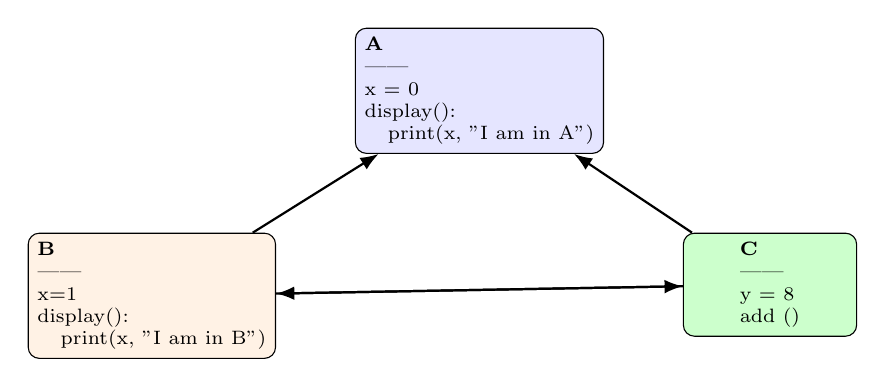
\begin{tikzpicture}[
  node distance=10mm and 10mm, % tighter spacing
  every node/.style={
    draw,
    rounded corners,
    align=center,
    font=\scriptsize,
    minimum width=2.2cm,
    minimum height=0.9cm 
  },
  arrow/.style={-Latex, thick}
]

\node[fill=blue!10, align=left] (A) {\textbf{A} \\ ------ \\ x = 0 \\ display(): \\ \hspace*{2mm} print(x, "I am in A") };
\node[fill=orange!10, align=left, below left=of A] (B) {\textbf{B} \\ ------ \\ x=1\\ display(): \\ \hspace*{2mm} print(x, "I am in B")};
\node[fill= green!20, align = left, below right = of A ] (C) {\textbf{C} \\ ------ \\ y = 8 \\ add () };

\draw[arrow] (B) -- (A);
\draw[arrow] (C) -- (A);
\draw[arrow] (C) -- (B);
\draw[arrow] (B) -- (C);
\end{tikzpicture}
\end{center}




\begin{algorithm}
\caption{Display Method Example}
\begin{algorithmic}
\STATE \textbf{Method} add(int a, int b)
\STATE \quad resuts $ \leftarrow a + b $
\STATE \quad return  results   


\end{algorithmic}

\end{algorithm}


\begin{lstlisting}[style=vscode]
class Car:
    def __init__(self, color, price):
        self.color = color
        self.price = price

    def getColor(self):
        return self.color

    def getPrice(self):
        return self.price

    def setPrice(self, price):
        self.price = price

car1 = Car("Red", 15000)
print(car1.getColor())
print(car1.getPrice())
\end{lstlisting}




\end{document}
